\documentclass[11pt,a4paper]{article}
\usepackage[utf8x]{inputenc}
\usepackage{ucs}
\usepackage{amsmath}
\usepackage{amsfonts}
\usepackage{amssymb}
\usepackage{url}
\usepackage{graphicx}
\usepackage{subfigure}

\newcommand{\question}{\textbf{---NEED-REVIEW-HERE---}}

\author{HU, Pili}
\title{Spectral Techniques for Community Detection on 2-Hop Topology}

\begin{document}

\maketitle

\begin{abstract}
	In one of our former project\cite{hu2011-cd2hop}, we formulated
	the problem of community detection on 2-hop topology. Given 
	one observer in a social network, and the graph it can reach 
	within two steps, we want to determine for those vertices whether they're
	in the same community with the observer. 
	The previous project extracts features like Common Neighbours, Ademic/Adar
	Score, Pagerank, and Personalized Pagerank, etc. Then several neural 
	networks are trained to combine those features. 
	Interested readers can refer to \cite{hu2011-cd2hop}
	for more information.  
	
	In this project, we augment our research based on the same settings. 
	Several spectral techniques are leveraged to tackle with the 2-hop 
	problem. For instance, spectral clustering may utilize the information 
	hidden in more eigen vectors. Other technique like personalized PageRank 
	can be studied with the budgeted learning context. 
	For data, codes, and other materials, please refer to 
	our open source repository\cite{hu2012-spectral2hop}. 
\end{abstract}

\pagebreak
\tableofcontents
\pagebreak

\section{Introduction}

\subsection{Problem}
Notations:
\begin{table}[htb]
	\centering
	\caption{Notations}
	\label{tbl:notation}
	\begin{tabular}{c|c}
	\hline
	Symbol & Explanation \\
	\hline
	$n$ & node number \\
	\hline
	$m$ & edge number \\
	\hline
	$A$ & adjacency matrix \\
	\hline
	$A_{ij}$ & 1 if node $i$ and node $j$ are directly \\
	& connected, 0 otherwise\\
	\hline
	$N(i)$ & neighbourhood of $i$, namely \\
	& $N(i) = \{j | A_{ij} = 1 \}$ \\
	\hline
	$d(i)$ & degree of node $i$ \\
	& $d(i) = \sum_{j}{A_{ij}}$ \\
	\hline
	$o$ & observer \\
	\hline
	$l_i$ & the real label of node $i$ \\
	\hline
	$L_i$ & the predicted label of node $i$ \\
	\hline
	$N2(i)$ & the 2-hop neighbours we study, defined as \\
	& $\cup_{j \in N(i) \cup \{i\}}{N(j)}$\\
	\hline
	\end{tabular}
\end{table}

Problem settings:
\begin{itemize}
	\item Give observer $o$. 
	\item Give the two hop topology, namely the $N2(o)$ and 
	the associated links. 
	\item Try to predict $L_i$ according to the above information. 
	\item Ground truth $l_i$ is directly crawled from the website. 
\end{itemize}

\subsection{Evaluation}

Our evaluation method distinguishes this work from many 
previous ones. Usual evaluation criterion is defining 
a certain quality functions, like\cite{aggarwal2011social} normalized cut, 
conductance, and modularity. Different research groups 
have their own taste and preference. 

The major problem is, those quality functions can reflect 
the accuracy of algorithms only to a limited extent. 
Let spectral clustering be an example. Luxburg\cite{von2007tutorial}
explains clustering using the notion of finding sets of nodes 
with small conductance in between. In this way, if conductance 
is selectd as the quality function, a good "clustering" is 
a natural consequence of spectral clustering algorithm. 

While those quality functions are simple and intuitive to 
facilitate theoretical study, they can not completely reflect the 
real application performance. In this work, we crawled ground truth
data from one SNS, thus we're able to evaluate the output 
against those crawled label. 

\subsection{Digest of Previous Results}

Overall speaking, we didn't get satisfying result in the previous project. 
The diffusion matrix after combining 9 features with neural network
always show a tradeoff between precision and recall. 

\begin{figure}[htb]
    \label{fig:subfigures}
    \begin{center}
        \subfigure[Common Neighbour]{%
            \label{fig:roc_sub_common}
            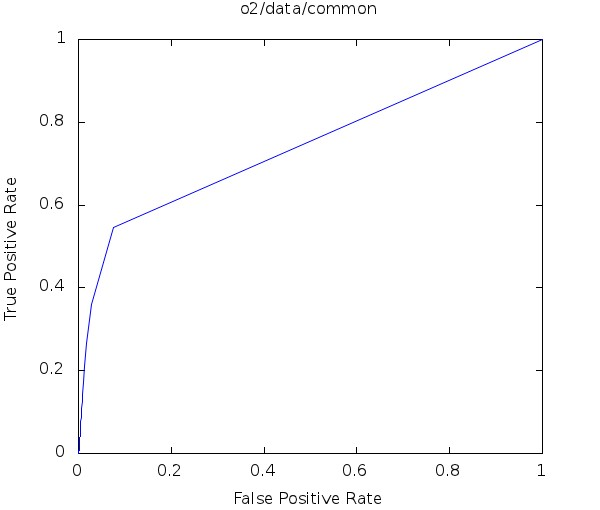
\includegraphics[width=0.3\textwidth]{../roc/pre-o2-fig/common.jpg}
        }%
        \subfigure[Ademic/Adar]{%
           \label{fig:roc_sub_adamic}
           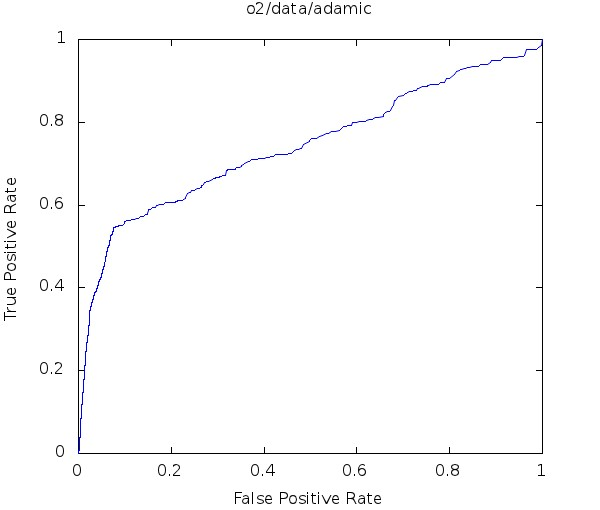
\includegraphics[width=0.3\textwidth]{../roc/pre-o2-fig/adamic.jpg}
        }
        \subfigure[Jaccard's]{%
            \label{fig:roc_sub_jacc}
            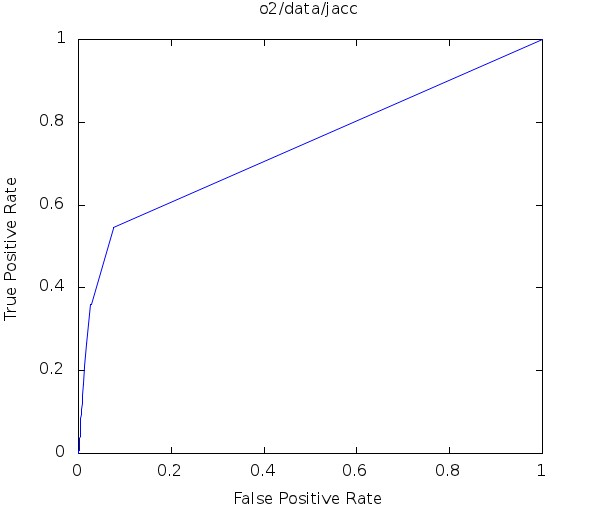
\includegraphics[width=0.3\textwidth]{../roc/pre-o2-fig/jacc.jpg}
        }\\%

        \subfigure[PR:EV=All 1's]{%
            \label{fig:roc_sub_pr_all1}
            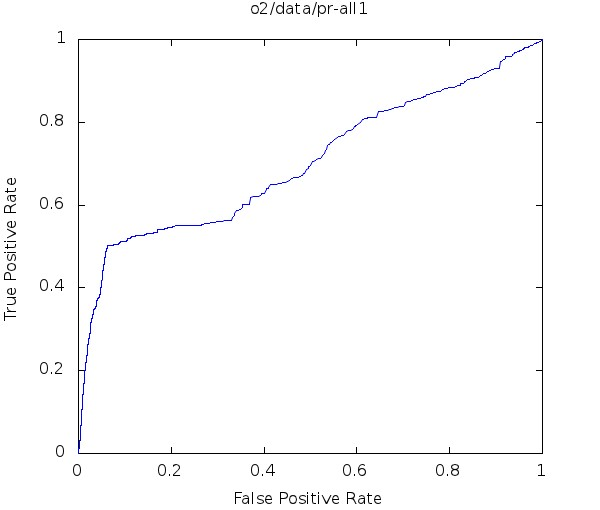
\includegraphics[width=0.3\textwidth]{../roc/pre-o2-fig/pr_all1.jpg}
        }%
        \subfigure[PR:EV=High 3]{%
           \label{fig:roc_sub_pr_high}
           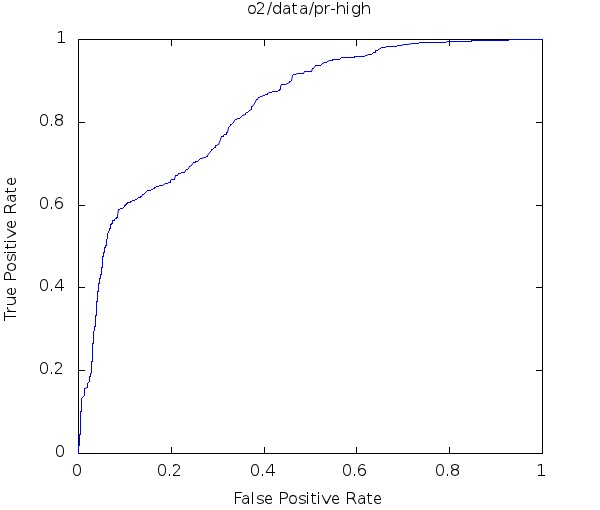
\includegraphics[width=0.3\textwidth]{../roc/pre-o2-fig/pr_high.jpg}
        }
        \subfigure[PR:EV=Root]{%
            \label{fig:roc_sub_pr_root}
            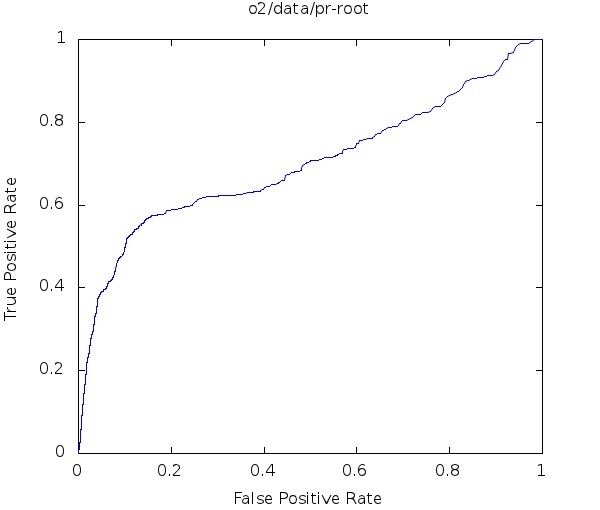
\includegraphics[width=0.3\textwidth]{../roc/pre-o2-fig/pr_root.jpg}
        }\\%
        
        \subfigure[PR:EV=All 1's(+SN)]{%
            \label{fig:roc_sub_pr_all1_super}
            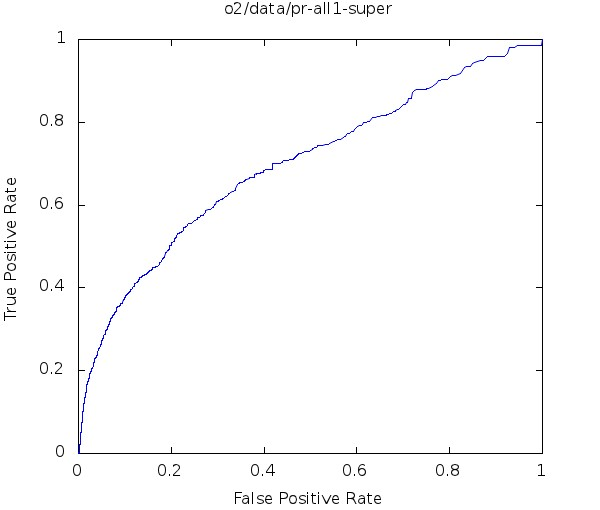
\includegraphics[width=0.3\textwidth]{../roc/pre-o2-fig/pr_all1_super.jpg}
        }%
        \subfigure[PR:EV=High 3 (+SN)]{%
           \label{fig:roc_sub_pr_high_super}
           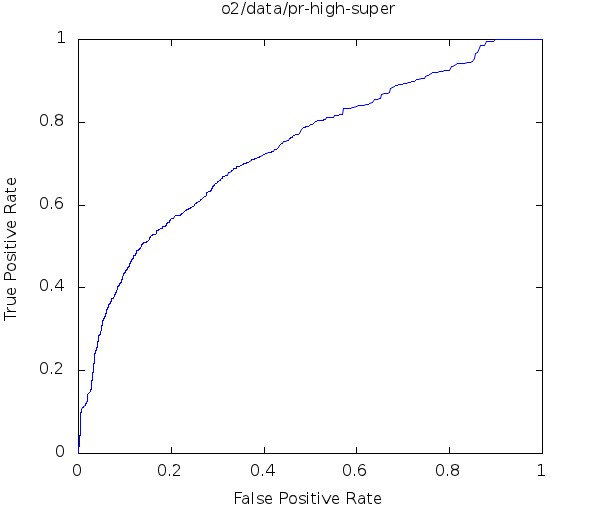
\includegraphics[width=0.3\textwidth]{../roc/pre-o2-fig/pr_high_super.jpg}
        }
        \subfigure[PR:EV=Root(+SN)]{%
            \label{fig:roc_sub_pr_root_super}
            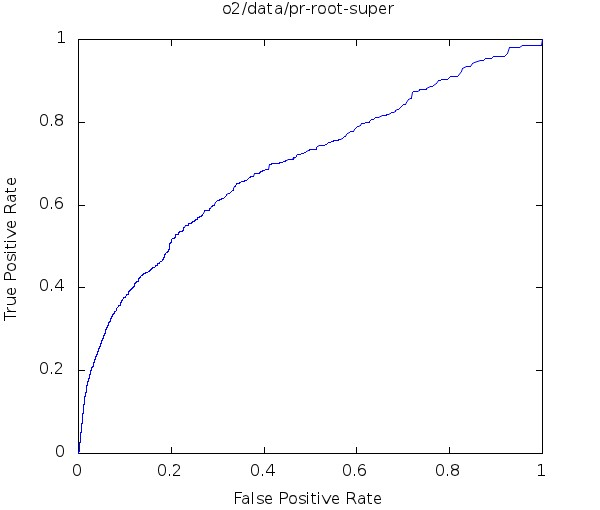
\includegraphics[width=0.3\textwidth]{../roc/pre-o2-fig/pr_root_super.jpg}
        }\\%
%
    \end{center}
    \caption{%
        ROC Curve of 9 Features
     }%
     \label{fig:old_roc_sub_all}
\end{figure}

Fig(\ref{fig:old_roc_sub_all}) shows the single feature evalutation result. 
By varying a threshold, we plot the True Positive Rate v.s. the False Positive 
Rate(label 1, namely "same community"). Those single feature evaluations 
are the useful part of the former project. The observations are:
\begin{itemize}
	\item Three simple features, as claimed by some researchers already 
	performs well in practice. 
	\item Compared with those simple features, more complicated PR
	series exhibits little benefit. 
	\item Among the 6 PR variations, the best performed one is Personalized
	PR with escape vector equal to 3 highest degree nodes from the target 
	community. 
\end{itemize}

\section{Proposed Future Study Line}

\subsection{Evaluation Modification}

From previous study, we find that diffusion matrix is not the most 
convenient way to do evaluation. The diffusion matrix is the final 
result, but highly depends on choice of parameters(may be trained 
weights in neural network). In this work, we want to leverage 
spectral techniques and do a in depth study of them. We find that 
ROC Area(ROCA), namely the area under ROC curve, is more convenient 
to compare. The larger this area, the better an algorithm performs. 
Intuitively speaking, ROCA can be regarded as the expectation of
precision w.r.t threshold, assuming the threshold is chosen at random
uniformly. 

Besides, the previous study finds that the number of leaf nodes is 
so large that they influence our evaluation. i.e. for a normal user 
with 400 buddies, there may be 100,000 nodes within two hop. Among 
the 100,000 nodes, there may be 7,000 nodes belonging to the same 
community with the observer. Under such situation, a naive algorithm 
assigning every node to label 0 can reach an accuracy of above 90\%. 
This outcome is of course not interesting at all. To evaluate the 
current work, we want to limit the scope of training and testing 
sets(full 2-hop topology is still served to algorithms). 

To conclude our evaluation method: 
\begin{itemize}
	\item Use ground truth rather than quality function. 
	\item Each algorithm outputs a "likelihood" value, 
	and we calculate ROCA by varying the threshold of this 
	likelihood value. 
	\item Full 2-hop topology is served to all algorithms, 
	but evaluation is done within a limited scope, like 
	only the level 1 nodes, without degree 1 nodes, etc. 
	Exact choice and justification will be provided in 
	the formal report. 
\end{itemize}

\subsection{Spectral Clustering}

Although we didn't use the term "spectral", we actually applied 
one very useful spectral technique, PageRank. To be short, variations 
of PR are all the principal eigenvector of a certain matrix. 
This value is shown to be informative for finding some local 
sparse cuts\cite{csci5160course}. 

As is known, there are much more eigenvectors that are not used in PR. 
It's no surprise that those successive eigenvectors can help to 
distinguish nodes from different clusters. Luxburg's tutorial\cite{von2007tutorial}
uses a simple example to illustrate this idea. 

Note one thing that although we talk "eigen vectors" in both paragraphs above, 
they corresponds to different matrix. In calculating PR, the matrix 
is obtained from (maybe weighted) adjacency matrix. However, in spectral 
clustering practice, people find the corresponding Laplacian is more useful. 

However, taking as many eigenvectors as possible may not be a good
idea. For one thing, computational cost is higher when dealing with 
more eigenvectors. For another thing, not all eigenvectors are informative. 
Luxburg\cite{von2007tutorial} provides some practical guides on the choice 
of number of eigenvectors. The eigen gap is taken into consideration as a 
general rule. However, bearing in mind that the current work is dealing 
with limited 2-hop topology, there can be proved to be definitely many 
non-informative eigenvectors. Spielman
gives a lemma in his lecture notes\cite{spielman-2009spectral-ln}:
\textbf{if two degree one nodes(say, $i,j$) have a common neighbour, there will 
be a eigen vector taking the $i$-th entry as 1 and $j$-th entry as -1}. 
In our case, large number of level 2 nodes can form this kind of pair. 
The computed eigenvectors may be a linear transformation of such 
standard vectors. The transformed version is also only able to distinguish 
node by node, carrying no cluster information. 

Chanllenges on this line:
\begin{itemize}
	\item How many eigenvector to use? 
	\item What's the number of clusters $k$ used in the 
	meta clustering? 
	\item How to do postprocessing to give final class labels? 
	\item Which form of Laplacian performs is preferred? 
	(Laplacian, Normalized Laplacian, One-side Normalized Laplacian)
	\item Any theoretical guarantee for the above issue? 
	(especially in the context of 2-hop)
\end{itemize}

\subsection{Personalized PR}

The general form of personalized PR is shown in eqn(\ref{eq:ppr}). 
\begin{equation}
	\vec{v} = \alpha A^{\rm T}\vec{v}
	+ (1-\alpha)\frac{\vec{b}}{||\vec{b}||_1}
	\label{eq:ppr}
\end{equation}

If we want to compute the PPR for a set of starting nodes, 
we only need to set all entries corresponding to those nodes 
to 1, and others are left zero. Of course, setting those non-zero
entries to values other than 1 is possible but in the current work 
we only consider 1 for simplicity(meaning no bias on the starting 
set). 

In this work, we'll do a survey on PPR related literature.
We seek for potential theoretical characterization of our problem, 
since in the former work we already find that PPR performs the best
alone. 

\subsection{Budgeted Learning}

In practice, resources are often limited, so we want to do 
budgeted learning. That is, finding the tradeoff between 
cost and performance. 

This research line roots from the observation on PPR:
\begin{itemize}
	\item PPR can be linearly combined:
\begin{eqnarray}
	\vec{v} &=& \alpha A^{\rm T}\vec{v}
	+ (1-\alpha)\frac{\vec{b}}{||\vec{b}||_1} \\
	&=& \alpha A^{\rm T}\vec{v}
	+ (1-\alpha)\frac{
	\sum_{i \in 
	\text{support($\vec{b}$)}}{e_i}}
	{||\vec{b}||_1} \\
	&=& \frac{1}{{||\vec{b}||_1}}
	\sum_{i \in \text{support($\vec{b}$)}}{\alpha A^{\rm T}\vec{v}_i}
	+
	\frac{1}{{||\vec{b}||_1}}
	\sum_{i \in \text{support($\vec{b}$)}}{(1-\alpha)e_i}
	\label{eq:ppr_linear} 
\end{eqnarray}
\end{itemize}


\subsection{Visualization}

\subsection{Cluster Ensemble}

\input{../reference/gen_bib.bbl}

\end{document}
